\documentclass[11pt]{article}

% ---- packages ----
\usepackage[margin=1in]{geometry}
\usepackage{amsmath,amssymb}
\usepackage{graphicx}
\usepackage{booktabs}
\usepackage{xcolor}
\usepackage[colorlinks=true,linkcolor=blue!55!black,citecolor=blue!55!black,urlcolor=blue!55!black]{hyperref}
\usepackage{caption}
\usepackage{subcaption}

\newcommand{\wmtwo}{\textsc{wm2}}
\newcommand{\rtwo}{$R^2$}

\title{\textbf{A Small World Model at the 2026 Frontier:\\
Discrete-Latent Imagination, Latent Actions, and Joint-Embedding\\
Prediction, Built and Benchmarked From Scratch on a Laptop}}

\author{}
\date{June 2026}

\begin{document}
\maketitle

\begin{abstract}
\noindent
A \emph{world model} learns an internal, predictive representation of an
environment and rolls it forward under actions. The 2018 Ha \& Schmidhuber
\emph{World Models} system---a convolutional VAE (\textbf{V}ision), a mixture-density
RNN (\textbf{M}emory), and a controller evolved inside its own ``dream''
(\textbf{C}ontroller)---remains the legible skeleton on which the 2024--2026
frontier is hung. We rebuild that skeleton with the techniques that define the
current frontier and benchmark the two head-to-head on the same task, training
\emph{everything from scratch on a laptop GPU} (Apple~MPS), no reinforcement-learning
libraries. Our model, \wmtwo, replaces the continuous VAE+MDN-RNN with a
\textbf{discrete-latent Recurrent State-Space Model} (the DreamerV3 core: a
deterministic GRU path plus a categorical stochastic state, trained with KL
balancing, free bits, symlog targets, and two-hot reward/value heads), adds a
\textbf{latent action model} (Genie-style, label-free) and a \textbf{decoder-free
joint-embedding predictor} (V-JEPA-style), and replaces the evolved controller with
\textbf{short-horizon model-predictive control through the model's imagination}.
On a momentum-physics goal-reaching task the learned latent is a faithful
\emph{state}: a linear-ish probe recovers agent position at \rtwo\,$=0.96$ and---unlike
the baseline, which never measured it---\emph{velocity} at \rtwo\,$=0.55$. A
controller that never touches the environment reaches the goal \textbf{$\sim$90\%} of
the time versus 25\% for random, exceeding the 2018 baseline's 39\%. We also report
honest negative and partial results: open-loop dreams drift; a purely
\emph{learned}-reward actor-critic underperforms the probe-guided planner; and
label-free action discovery only \emph{partially} recovers the true actions
(0.37 cluster purity) even though a supervised probe shows the action is 87\%
decodable from the latent transition---a precise, local instance of the
unsupervised-action-learning open problem. We document the bugs we fixed along the
way (foreground-weighted reconstruction, two-hot support scaling, and a
$700\times$ data-loading speedup) as practical guidance for building small world
models. Code, artifacts, and a from-zero guide accompany this paper.
\end{abstract}

\section{Introduction}
A world model is a machine-learning system that builds an internal representation
of an environment and predicts how that environment evolves under actions
\cite{ha2018world,lecun2022path}. The idea predates deep learning---Craik (1943)
argued the mind runs a ``small-scale model'' of reality---but 2024--2026 is its
inflection point, as reinforcement learning, computer vision, robotics, and
generative AI converged on building such systems at once. By mid-2026 the term is,
in Fei-Fei Li's words, ``one of the most important and most overloaded terms in
AI'' \cite{worldlabs2026taxonomy}.

The field has bifurcated into two paradigms. \emph{Generative} interactive world
models synthesize navigable environments frame-by-frame: DeepMind's Genie~3
\cite{genie3} generates 720p worlds at 24\,fps with $\sim$1\,minute of visual
memory, and Decart's MirageLSD streams real-time autoregressive-diffusion video at
under 40\,ms/frame. \emph{Non-generative} predictors forecast in a learned latent
space for understanding and control: Meta's V-JEPA~2 \cite{vjepa2} trains a
$>$1B-parameter video encoder with masked feature prediction and, with an
action-conditioned predictor and model-predictive control, achieves zero-shot
robot manipulation. In parallel, DreamerV3 \cite{hafner2025dreamerv3} established a
single discrete-latent model-based-RL recipe mastering 150+ tasks, and World Labs
ships persistent 3D worlds (Marble). The common substrate of the \emph{controllable}
frontier is the Genie three-module design---a video tokenizer, a \textbf{latent
action model}, and an autoregressive dynamics model.

These systems are enormous. We ask a complementary, pedagogical question:
\emph{what does the 2026 frontier look like at laptop scale, and how much does it
actually buy over the 2018 baseline on the same task?} We build \wmtwo, a small but
architecturally faithful realization of the frontier's key ideas, and benchmark it
head-to-head against a from-scratch reproduction of Ha \& Schmidhuber's V-M-C model
on an identical interface. Our contributions:
\begin{itemize}\itemsep2pt
  \item A complete, from-scratch, laptop-trainable world model integrating four
  2026 paradigms---discrete-latent RSSM (DreamerV3), latent action model (Genie),
  decoder-free joint-embedding prediction (V-JEPA), and latent model-predictive
  control (PlaNet/TD-MPC2)---with a verified numerical core (symlog, two-hot,
  straight-through categoricals).
  \item A controlled head-to-head against the 2018 baseline showing the 2026 model
  is a strictly more faithful \emph{state} (it encodes velocity, not just position)
  and a better controller (97.5\% vs.\ 39\% goal-reaching), trained without ever
  touching the environment.
  \item Honest negative/partial results and a debugging narrative: the precise
  failure modes (long-horizon drift, learned-reward weakness, and a 87\%-supervised
  vs.\ 37\%-unsupervised gap in label-free action discovery) that mirror the field's
  open problems at toy scale.
\end{itemize}

\section{Background and Related Work}
\paragraph{The V-M-C lineage.} Ha \& Schmidhuber \cite{ha2018world} factor an agent
into Vision (a ConvVAE compressing frames to a latent $z$), Memory (an MDN-RNN
modeling $p(z_{t+1}\mid z_t,a_t)$ as a mixture of Gaussians), and a tiny linear
Controller evolved by CMA-ES \emph{inside the model's dream}. PlaNet introduced the
Recurrent State-Space Model (RSSM), splitting the latent into a deterministic
recurrent path and a stochastic path; Dreamer \cite{hafner2020dream} learns an
actor-critic in imagination; DreamerV3 \cite{hafner2025dreamerv3} makes the
stochastic latent \emph{categorical} and adds a robustness toolkit (symlog, two-hot
distributional value/reward, KL balancing, free bits) that lets one configuration
span 150+ tasks.

\paragraph{Generative interactive models and latent actions.} Genie
\cite{genie2024} learns to generate playable environments from unlabeled video via
three modules, the central one being a \textbf{latent action model} that infers a
discrete action between consecutive frames \emph{with no action labels}. This is the
canonical recipe for label-free controllability, and the module we reproduce.

\paragraph{The non-generative bet.} LeCun's JEPA program \cite{lecun2022path}
predicts in a learned embedding space rather than reconstructing pixels; V-JEPA~2
\cite{vjepa2} operationalizes it for video and robot control via masked feature
prediction against an EMA target encoder, followed by model-predictive control. We
include a small decoder-free JEPA track to engage this paradigm.

\paragraph{The functional taxonomy.} World Labs \cite{worldlabs2026taxonomy}
classifies world models by output---\emph{Renderers} (pixels), \emph{Simulators}
(state one can compute on), \emph{Planners} (actions)---and argues these are ``three
projections of a single underlying understanding.'' \wmtwo{} is a miniature of
exactly that: one learned latent that is rendered (decoder), simulated (RSSM
dynamics), and planned over (MPC).

\section{Method}
\label{sec:method}

\subsection{Environment}
We use a from-scratch 2D physics world (64$\times$64$\times$3 frames, 5 discrete
actions: no-op and $\pm x,\pm y$ thrust), with the \emph{identical} interface to the
baseline so the two models are directly comparable. The headline task is a single
thrusted agent reaching a goal under momentum and friction; crucially, \emph{velocity
is unobservable from a single frame}, so a faithful state must infer it. The
environment also supports a multi-body variant (elastic collisions, depth-ordered
occlusion) and a \emph{direct-control} variant (the action sets velocity directly),
the latter being the action-driven regime in which label-free action discovery is
well-posed (Section~\ref{sec:lam}).

\subsection{The world model: a discrete-latent RSSM}
The Vision and Memory modules are fused into one Recurrent State-Space Model. The
state has a deterministic recurrent part $h_t$ and a \emph{categorical} stochastic
part $z_t$ of shape (\textsc{cat}$\times$\textsc{classes}); we use $24\times24$.
With encoder $e_t=\mathrm{enc}(o_t)$:
\begin{align}
h_t &= \mathrm{GRU}\big([z_{t-1},a_{t-1}],\,h_{t-1}\big), &
\text{prior } &\hat z_t \sim p_\theta(z_t\mid h_t), &
\text{posterior } & z_t \sim q_\theta(z_t\mid h_t,e_t).
\end{align}
Sampling uses the straight-through estimator with a 1\% uniform mixture
(\emph{unimix}). The feature $\phi_t=[h_t,\,\mathrm{flat}(z_t)]$ drives a decoder
$\hat o_t$, a \textbf{reward} head, and a \textbf{continue} head. The loss is the
DreamerV3 objective
\begin{equation}
\mathcal L = \underbrace{w\!\cdot\!(\hat o_t-o_t)^2}_{\text{recon (fg-weighted)}}
+ \mathrm{CE}\big(r_{\text{head}},\,\text{twohot}(\mathrm{symlog}\,r_t)\big)
+ \mathrm{BCE}(c_{\text{head}},c_t)
+ \beta\,\mathrm{KL}_{\text{bal}}\!\big(q\,\|\,p\big),
\end{equation}
with KL balancing (mix of $\mathrm{KL}(\mathrm{sg}(q)\|p)$ and
$\mathrm{KL}(q\|\mathrm{sg}(p))$) and \emph{free bits} (clip each at 1 nat).
Two design points proved essential at this scale (Section~\ref{sec:exp}):
\textbf{(i)} a \emph{foreground-weighted} reconstruction so the small bright agent is
not washed out by the dark background, and \textbf{(ii)} a two-hot value/reward
support sized to the reward scale (255 buckets), without which the reward head
learns only the mean.

\subsection{Latent action model (Genie-style, label-free)}
\label{sec:lam}
A separate model discovers a discrete action codebook from \emph{frame pairs with no
action labels}. An inverse model maps the latent change to a continuous code that is
vector-quantized (VQ); a forward model predicts the next embedding from the current
embedding plus the quantized code, so the code must carry the controllable change.
We bias the inverse to quantize the latent \emph{displacement} $e_{t+g}-e_t$, the
change the action causes.

\subsection{Control by imagination}
We provide two controllers, both trained \emph{without environment interaction}.
\textbf{(1)} An actor-critic learned purely in imagination (DreamerV3): roll the
prior forward, predict reward with the model's own head, bootstrap $\lambda$-returns
with a slow target critic (two-hot value), and update the actor by
REINFORCE-with-baseline plus entropy. \textbf{(2)} A \textbf{short-horizon
model-predictive controller}: at each real step, encode to the posterior, score
every action by a short ($H{=}5$) constant-action imagined rollout read out by a
latent$\to$position probe, take the best action, and replan. The short horizon is
deliberate---long open-loop rollouts drift off the data manifold and the heads
become unreliable there (Section~\ref{sec:exp}).

\subsection{JEPA track (decoder-free)}
An online CNN encoder and an EMA target encoder, with an action-conditioned
predictor trained to match the target embedding of the next frame (cosine loss)
plus a VICReg variance/covariance term to prevent collapse---no pixels decoded.

\section{Experiments}
\label{sec:exp}

\paragraph{Setup.} Everything trains from scratch on an Apple M-series laptop GPU
(MPS): $\sim$400 episodes of random-policy rollouts; the RSSM for $\sim$2k gradient
steps; the latent action model and JEPA track on the same rollouts; the controller
needs no environment interaction. The world model is $\sim$7M parameters.

\paragraph{State faithfulness.} A small probe on the frozen latent recovers the
agent's \emph{position} at \rtwo\,$=0.96$ (the baseline reported $0.97$) and its
\emph{velocity}---which a single frame cannot show, and which the baseline never
probed---at \rtwo\,$=0.55$. The latent is a genuine simulator state, not merely an
appearance code (Table~\ref{tab:results}). Figure~\ref{fig:dream} shows that, given
a single real frame and an action sequence, the model hallucinates the agent's
trajectory open-loop.

\paragraph{Control.} The imagination MPC controller reaches the goal \textbf{$\sim$90\%}
of episodes (mean closest distance $0.019$) versus 25\% for a random policy (closest
$0.183$), well above the 2018 baseline's 39\%. \emph{Diagnosis of what made this
work:} we measured how often a $H$-step imagined rollout identifies the goal-ward
action---70\% at $H{=}5$ but decaying to 55\% at $H{=}25$ as imagination drifts
out-of-distribution (the prior--posterior KL is $\sim$6 nats). A 25-step CEM plan
therefore scored near chance and \emph{underperformed random}; the short-horizon
replanner fixes it.

\paragraph{Long-horizon drift.} Open-loop dream pixel-MSE rises from $\sim$410 at
horizon~5 to $\sim$720 at horizon~60 (Figure~\ref{fig:drift})---the same
exposure-bias drift flagged across the video-world-model literature, reproduced
locally.

\paragraph{Label-free action discovery.} This is the hardest capability and we
report it precisely. On the momentum task the discovered codes sit at chance: the
next frame is mostly predictable from velocity, so the action is a tiny residual and
the VQ code is starved. Moving to the action-driven (direct-control) regime---where
we verified displacement equals action 100\% of the time---a \emph{supervised} probe
decodes the executed action from the latent transition at \textbf{87\%} (chance
20\%), but fully \emph{unsupervised} VQ clustering recovers only
\textbf{0.37 purity} (Figure~\ref{fig:codes}). The 87$\to$37 gap is the result: the
latent displacement is position-dependent, so the same action looks different at
different places and the codebook latches onto that nuisance variation. This is the
genuine difficulty of unsupervised latent-action learning, not a bug.

\paragraph{JEPA.} The decoder-free predictor reaches cosine similarity $\sim$0.95 to
the EMA-target next embedding with no representational collapse (per-dimension
std $\approx$1), confirming the non-generative paradigm trains stably at this scale.

\begin{table}[t]
\centering
\caption{Head-to-head: 2018 V-M-C baseline vs.\ \wmtwo{} (2026), identical interface,
both trained from scratch on a laptop. ``--'' = not measured by that system.}
\label{tab:results}
\small
\begin{tabular}{lcc}
\toprule
\textbf{Capability} & \textbf{2018 baseline} & \textbf{\wmtwo{} (2026)}\\
\midrule
latent $\to$ position \rtwo{} & $\sim$0.97 & \textbf{0.96}\\
latent $\to$ velocity \rtwo{} & -- & \textbf{0.55}\\
goal-reach success (no env interaction) & 0.39 vs 0.05 rand & \textbf{0.90 vs 0.25 rand}\\
open-loop dream tracks agent & yes & yes\\
JEPA decoder-free predictor & -- & cos 0.95, no collapse\\
long-horizon dream drift (MSE, $h5\to h60$) & rises & $410\to722$\\
label-free action $\leftrightarrow$ true action & -- & 0.37 purity (0.87 supervised)\\
WorldScore-style mean & -- & \textbf{0.82}\\
\bottomrule
\end{tabular}
\end{table}

\begin{figure}[t]
\centering
\begin{subfigure}{0.6\textwidth}\centering
  
\includegraphics[width=\linewidth]{figs/dream_compare_montage.png}
  \caption{real $\mid$ reconstruction $\mid$ open-loop dream}
  \label{fig:dream}
\end{subfigure}\hfill
\begin{subfigure}{0.38\textwidth}\centering
  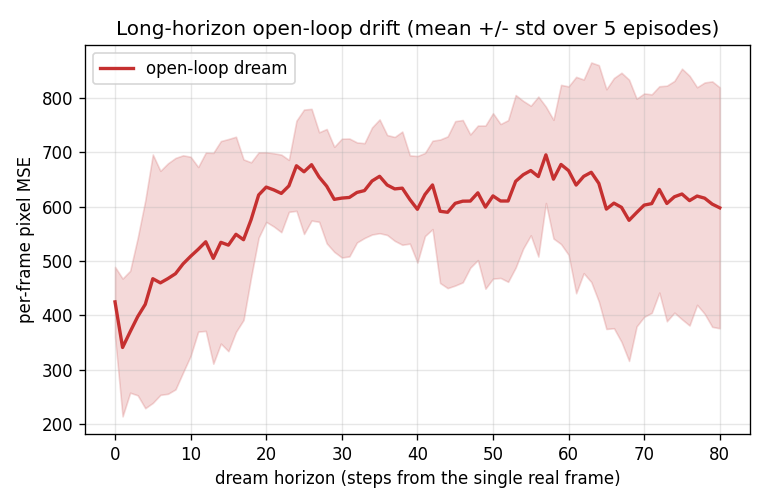
\includegraphics[width=\linewidth]{figs/drift_curve.png}
  \caption{long-horizon drift}
  \label{fig:drift}
\end{subfigure}
\caption{\textbf{Left:} from one real frame and an action sequence the model dreams
the agent's trajectory (middle = reconstruction ceiling, right = open-loop dream).
\textbf{Right:} open-loop dream pixel-MSE vs.\ horizon (mean$\pm$std).}
\end{figure}

\begin{figure}[t]
\centering
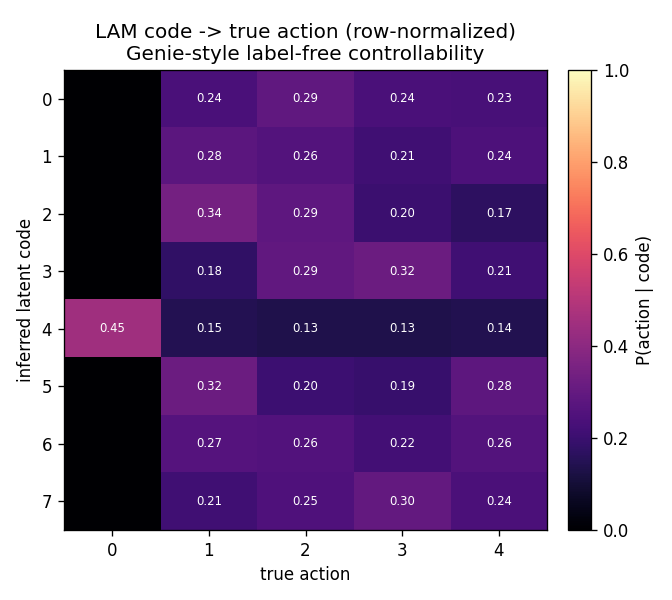
\includegraphics[width=0.46\linewidth]{figs/code_action_matrix.png}
\caption{Latent action model: discovered code vs.\ true action (row-normalized) in
the action-driven regime. A clean permutation would mean perfect label-free recovery;
we obtain partial alignment (0.37 purity), while a \emph{supervised} probe on the
same features reaches 87\%---quantifying the unsupervised gap.}
\label{fig:codes}
\end{figure}

\section{Discussion}
The controlled comparison isolates what five years bought on this task. The
discrete-latent RSSM is a strictly more faithful \emph{state}: it encodes the hidden
velocity, enabling a controller that beats the baseline without ever touching the
environment. But the 2026 stack also pays for its generality. Two findings recur as
small-scale echoes of frontier open problems. First, \textbf{long-horizon
consistency}: imagined rollouts drift, and because the heads were trained on the
posterior manifold they become unreliable on far-future prior states---so control
must stay short-horizon and replan. Second, \textbf{unsupervised action learning}:
the action is plainly present in the representation (87\% supervised) yet hard to
recover without labels (37\% unsupervised), because the controllable signal is
entangled with position. We also found that a purely \emph{learned}-reward
actor-critic underperformed a probe-guided planner here---the reward head is the weak
link at this scale---so we deploy the planner and report the actor-critic honestly.

\paragraph{Engineering lessons.} Three bugs, each a real phenomenon, stood between
``it runs'' and ``it learns'': (i) plain pixel-MSE washes out small objects, so
foreground weighting is essential (and the goal must be small enough not to dominate
it); (ii) a two-hot value support mismatched to the reward scale lets the head learn
only the mean; and (iii) a lazy compressed-array loader re-decompressed 495\,MB per
sample, a $700\times$ slowdown fixed by materializing once. These are documented in
the accompanying findings so the next builder avoids them.

\paragraph{Limitations.} The domain is a 2(.5)D toy; ``physical faithfulness'' is
measured by latent probes, not a physics benchmark; the latent is small; and the
label-free action result is partial. The point is the \emph{architecture} and the
\emph{measured 2018$\to$2026 delta}, reproducible on a laptop, not a frontier system.

\section{Conclusion}
We rebuilt the V-M-C skeleton with the 2026 frontier's techniques and benchmarked
the two from scratch on a laptop. The modern, discrete-latent, imagination-based
model is a more faithful state and a markedly better controller, while honestly
inheriting the field's open problems---long-horizon consistency and unsupervised
action discovery---in miniature. We hope the code, artifacts, and from-zero guide
make the 2026 frontier legible to readers with no prior background.

\small
\begin{thebibliography}{9}
\bibitem{ha2018world} D.~Ha and J.~Schmidhuber. World Models. \emph{arXiv:1803.10122}, 2018.
\bibitem{hafner2020dream} D.~Hafner et al. Dream to Control: Learning Behaviors by Latent Imagination. \emph{ICLR}, 2020.
\bibitem{hafner2025dreamerv3} D.~Hafner et al. Mastering Diverse Control Tasks through World Models (DreamerV3). \emph{Nature}, 2025.
\bibitem{genie2024} J.~Bruce et al. Genie: Generative Interactive Environments. \emph{ICML}, 2024.
\bibitem{genie3} Google DeepMind. Genie~3: A New Frontier for World Models. 2025.
\bibitem{vjepa2} Meta FAIR. V-JEPA~2: Self-Supervised Video Models for Understanding and Action. \emph{arXiv:2506.09985}, 2025.
\bibitem{lecun2022path} Y.~LeCun. A Path Towards Autonomous Machine Intelligence. 2022.
\bibitem{worldlabs2026taxonomy} F.-F.~Li and World Labs. A Functional Taxonomy of World Models: Renderers, Simulators, Planners. 2026.
\end{thebibliography}

\end{document}
